%***************************************************************************
% XSPIF user's guide -  userguide.tex
% Chapter : From the model to the XML description
% Authors: Remy Muller & Vincent Goudard
%***************************************************************************

\chapter{From the model to the XML description}


\section{The model}

\noindent Here is a simple model behind audio plugins architecture. A
plugin can be viewed as a kind of black box, which gets audio buffer(s)
and control value(s) as inputs, and outputs transformed audio buffer,
and control values. 

\begin{figure}[htb]
\begin{center}
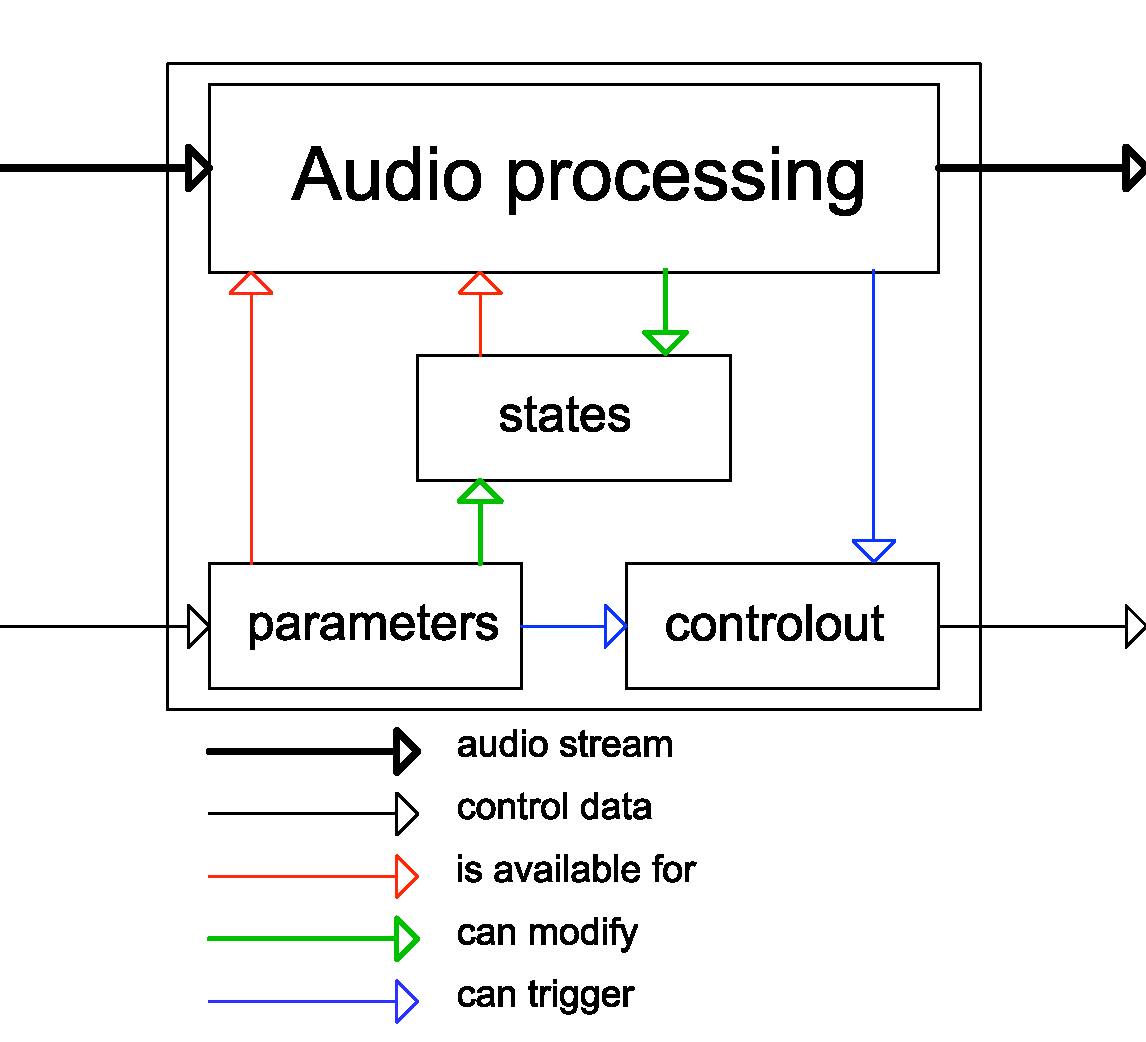
\includegraphics[height=3.5in,width=3.5in]{pluginmodel}
\caption{XSPIF model behind audio plugins}\label{xspifpluginmodel}
\end{center}
\end{figure}

\noindent However, as long as our plugin remains a model, it will not do much.\\
\noindent In order to perform its job, this box needs to be \emph{instanciated}. Instanciation consists in allocating the memory needed by the plugin and its variables.\\
\noindent Then it needs to be \emph{activated}, i.e. perform and
compute everything that is needed, so that the plugin is ready to perform some DSP processing.\\
\noindent If we want to stop processing audio for a while, we can
\emph{deactivate} the plugin, just like we would do with an on/off (or
bypass) switch for a machine.\\
\noindent Now, when we no longer want to use this plugin, we have to
\emph{deinstantiate} to free the memory location used by the plugin,
and by the structure it needs.\\
\noindent To sum up what is said above, we've introduced the
following \textbf{callbacks} (i.e. the methods of the plugin that you
can implement.):
\begin{itemize}
\item \textbf{instantiate}: the constructor.
\item \textbf{deinstantiate}: the destructor.
\item \textbf{activate}: plugin ON.
\item \textbf{deactivate} plugin OFF (bypass).
\item \textbf{process} where the DSP algorithm is implemented.
\end{itemize}

\section{Document Type Definition}

\noindent This very raw and simple model led us to a XML meta-plugin description 
with various elements. The Document Type Definition \verb|xspif.dtd| is a file 
describing the way a meta-plugin should be written.\\
\noindent More precisely it defines what the possible or required
elements are, where they are, how many of them one can find in the
meta-plugin, what are their attributes and sub-elements and what value
they can take.\\ 
\noindent The user can refer to this file to get a quick overview of
the meta-plugin syntax. Otherwise refer to the next section \ref{tutorial} which will explain in details all the elements you can use and their respective roles.  

\section{XML syntax}

\noindent XML\footnote{XML: eXtended Markup Language}\cite{Walsh} is  
language to describe documents containing structured information. 
The information in embedded in \emph{elements} defined by an opening 
and a closing \emph{tag}:\\
$<myElement> ... information ... </myElement>$

\noindent These elements can have \emph{child elements}, as well as
\emph{attributes} -- some information specific to the element --
The various elements used in XSPIF are listed below, and 
further described in the next chapter:

\begin{tabular}{l|l}
Elements                                     & Signification \\
\hline
$<plugin  (attributes)> </plugin>$           & Main element\\
$<pin  (attributes)> </pin>$                 & Audio input or output\\
$<param  (attributes> </param>$              & Controllable parameter\\
$<state  (attributes)> </states>$            & Internal state\\
$<controlout  (attributes)> </controlout>$   & Control output\\
$<caption> </callback>$                      & Caption of the parent element\\
$<comment> </callback>$                      & Comment for the parent element\\
$<code> </callback>$                         & Code for the parent element\\
\end{tabular}